\chapter{ScriptButler}
\label{ch:research}
Here we present ScriptButler, a prototype tool for analyzing PuzzleScript games. The tool aims to give game designers a better understanding of how code changes affect gameplay. As previously mentioned, we created this prototype because the official PuzzleScript implementation is unsuitable for our research goals. Therefore, to resolve this issue we create our own design and implementation of PuzzleScript. We base our implementation on the design document we reverse engineered in the previous chapter. In this chapter, we discuss the design decisions we take. Our aim with this implementation is to create a general-purpose tool capable of parsing, validating, and running games. Additionally, for the purpose of this project, we also design a dynamic analysis module to provide support for analyzing gameplay. The dynamic analysis module also demonstrates the extensibility of our prototype.

Figure \ref{fig:scriptbutler_flow} shows an overview of our tool's architecture. The game designer interact with the tool through the IDE and the Web GUI. These two components provide user-friendly endpoints to our tool and are responsible for sending inputs from the game designer to the tool. ScriptButler is split up into multiple phases, this is done to reduce issues tied to coupling. The parser is our grammar, it reads PuzzleScript code and converts it into Rascal data structures. The post-process phase cleans up those data structures and annotates them to provide an outline and syntax coloring. The static checker verifies the validity of the code and provides error messages that the IDE can display to the game designer. The compiler further transforms the data structures, removing unnecessary content and making them more efficient to run in our engine. The engine run the game and displays the result in the Web GUI. The user can send inputs to the engine using that GUI and get debugging information. Finally, the dynamic analyzer runs tests on the compiled version of the game and provides feedback on the gameplay as messages that the IDE can display. We explain all the sections in greater detail in the following sections. 

\begin{figure}[!t]
    \centering
    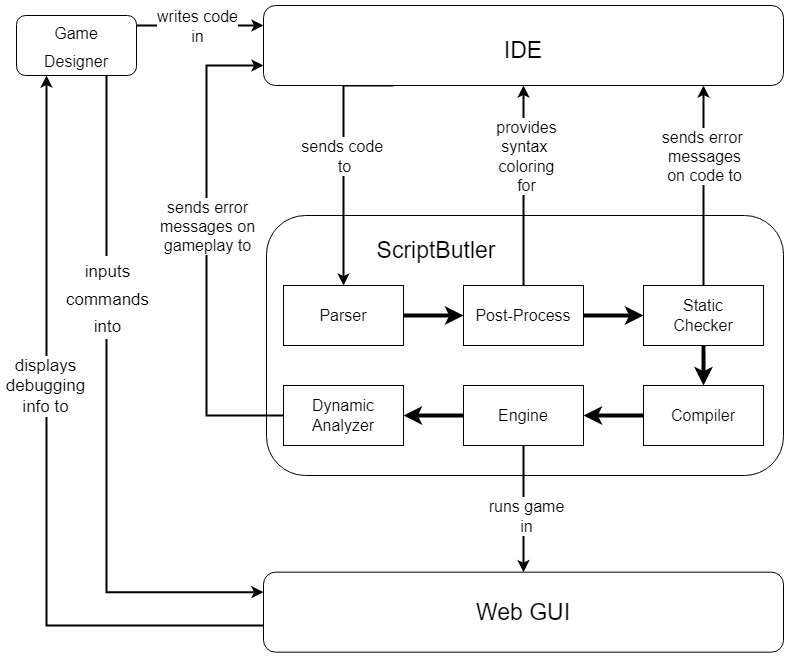
\includegraphics[width=1\textwidth]{images/ScriptButler Flow.png}
    \caption{The data flow through ScriptButler and its extensions}
    \label{fig:scriptbutler_flow}
\end{figure}

\section{Redesigning PuzzleScript with Rascal}
\newcommand{\dd}{\textsuperscript{[D]}}
Here we present the design of the PuzzleScript implementation we created using the design document we obtained by reverse-engineering the JavaScript implementation. Design decisions that arise from that understanding and that differ from the design decisions of the original implementation are marked with "\dd". When designing the implementation, we use a test-driven approach. We write the tests and their expected results based on the reverse engineering of the original implementation. We then implement PuzzleScript's design and frequently test our implementation against the tests. One of the goals for our implementation is to be compatible with existing games and the tests ensure we keep in line with that goal.

Our second goal is to create a design that is more maintainable than the original JavaScript one. Rascal satisfies part of that goal as a statically typed language. This makes it easier for programmers to understand the data flow. We also leverage good engineering practices such as self-documentation through the use of relevant variables and function names. Our third and final goal is creating an extensible design. To achieve this, we design our implementation with loose coupling between modules. Instead of creating a monolithic structure, we create a collection of plugins that are handled by a general function in charge of passing the data from one plugin to the other. Our approach makes it easy to add, remove or modify plugins. In the rest of this chapter, these plugins are called phases as they mirror, to an extent, the phases of compilation.

We split up the design of our implementation into separate phases\dd. Each phase has progressively stricter requirements on what counts as valid code. The phases are the following:
\begin{itemize}
    \item Parsing: Using a flexible formalized grammar, a PuzzleScript file is read and transformed into a parsed tree
    \item Post-process: The parsed tree is cleaned up and enriched with meta-data
    \item Static Check: Components of the file are checked for validity according to the specifications extracted from the JavaScript implementation.
    \item Compilation: The game is compiled into a form the engine can run, converting the AST to more efficient Rascal data structures
    % \item Dynamic Check: By running sections of the game using the engine, additional messages are generated on the gameplay
    \item Run: The game is running, allowing for the player to interact with it
    % \item Post-game analysis: Stats collected during the running phase are displayed
\end{itemize}

Splitting the compilation process into separate phases enables us to parse invalid code without the process aborting at the first error. The behavior assists designers in identifying multiple issues simultaneously.  We also separate the backend (parsing, checking, compiling) from the frontend (editor, interface)\dd. The backend is designed to accept source code, generate the data structures, and alter those data structures based on user input. The front end acts as a wrapper around the backend, communicating through specific endpoints. The approach allows us to decouple the user interface and engine, making it easier to alter either without impacting the other. Developers can even create their own implementation of the frontend or backend with seamless integration.

The design document of PuzzleScript is subject to errors of misinterpretation because it is based on reverse engineering. We mitigate these interpretation issues by verifying the design of our implementation against the behaviors of the official implementation. We go further into our verification process in Section \ref{sec:testing}.

\subsection{Parsing}
We address the need for a reusable and maintainable parser by creating a formal syntax definition in the form of a grammar. In our design, we make several important changes to this phase. However, we want our redesign to remain compatible with the PuzzleScript design. As such, it is important that this phase's user-facing endpoints do not change. The main design change in this phase is that we switch from using a hand-crafted parser to using Rascal's Syntax Definition feature\footnote{\url{https://docs.rascal-mpl.org/stable/RascalConcepts/\#RascalConcepts-SyntaxDefinitionAndParsing}}\dd. This decision allows us to create a declarative representation of a PuzzleScript file that consists of lexicals and symbols. This representation is human-readable and easier to extend than a line-based parser. 

A Rascal syntax definition consists of a layout, keywords, lexicals, and symbols. The layout is a pattern that matches the white space and comments, it can be seen at the top of Figure \ref{fig:PuzzleScript Lexicals}. Symbols are composed of lexicals, literals, and other symbols. We use lexicals to parse individual tokens and then group them into symbols that represent PuzzleScript components such as Objects, Rules, Sprites and many more. Figure \ref{fig:syntax_example} shows a simple example using practically all Syntax Definition features.

\begin{figure}[!t]
\begin{lstlisting}[language=rascal]    
// layout is lists of whitespace characters
layout MyLayout = [\t\n\ \r\f]*;

// identifiers are characters of lowercase alphabet letters, 
// not immediately preceded or followed by those (longest match)
// and not any of the reserved keywords
lexical Identifier = [a-z] !<< [a-z]+ !>> [a-z] \ MyKeywords;

// this defines the reserved keywords used in the definition of Identifier
keyword MyKeywords = "if" | "then" | "else" | "fi";

// here is a recursive definition of expressions 
// using priority and associativity groups.
syntax Expression 
  = id: Identifier id
  | null: "null"
  | left multi: Expression l "*" Expression r
  > left ( add: Expression l "+" Expression r
         | sub: Expression l "-" Expression r
         )
  | bracket "(" Expression ")"
  ;
\end{lstlisting}
\vspace*{-8pt}
\caption{Syntax example}
\label{fig:syntax_example}
\end{figure}

The main weakness of using Syntax Definition is that we lose control over how the parser handles invalid code. If the parser runs into invalid code it raises an error intended for the tool designer. This error is hard to read for the tool user and does not provide the necessary feedback for a game designer to fix their code. To address this issue, we create a \emph{'flexibile'} grammar. This means that our grammar should parse and accept invalid code, to an extent. We aim to design our grammar so that only severe structural errors can cause it to raise an error. To this end, we define keywords to make our definition more human-readable. However, we do not use them to exclude tokens to avoid a parser error. Our grammar is mostly made up of flexible lexicals grouped up under symbols. The main goal of our grammar is to assign "labels" to tokens so that our static checker knows what rules they should be checked against. Figure \ref{fig:PuzzleScript Lexicals} shows the lexicals, and Figure \ref{fig:example_symbol} shows a sample of our grammar that parses Objects. The latest version of the full grammar can be accessed on the project repository\footnote{\url{https://github.com/ClementJ18/ScriptButler/blob/main/src/PuzzleScript/Syntax.rsc}}.

The Syntax Definition also offers an opportunity to annotate the file with interesting metadata. This metadata can then be used by the syntax checker or IDE plugins to enrich and support the developer experience. For example, the \texttt{@Foldable} tag, allows the developer to collapse any piece of code that matches the symbol in the IDE to temporarily hide it. The design of our grammar does still present weaknesses. PuzzleScript's design presents several ambiguities which a formal grammar cannot handle. We mitigate the effect of these ambiguities by defining certain objects more rigidly. This approach directly counteracts our goal of keeping the grammar flexible so we carefully balance the two. 

The result of this section is a grammar that we can apply directly to a PuzzleScript file to generate a parse tree representing that game. The parse tree needs further manipulation to be usable but using a Syntax Definition fulfills our goal of creating a more readable version of PuzzleScript's grammar.

\begin{figure}[!t]
\begin{lstlisting}[language=rascal]
lexical LAYOUT 
	= [\t\r\ ]
	| ^ Comment Newlines
	> Comment
	;
layout LAYOUTLIST = LAYOUT* !>> [\t\r\ )];

lexical SectionDelimiter = [=]+ Newlines;
lexical Newlines = Newline+ !>> [\n];
lexical Comment = @Category="Comment" "(" (![()]|Comment)+ ")";
lexical Newline = [\n];
lexical ID = @Category="ID" [a-z0-9.A-Z#_+]+ !>> [a-z0-9.A-Z#_+] \ Keywords;
lexical Pixel = [TRUNCATED];
lexical LegendKey = Pixel+ !>> [TRUNCATED] \ Keywords;
lexical Spriteline = [0-9.]+ !>> [0-9.] \ Keywords;
lexical Levelline = Pixel+ !>> Pixel \ Keywords;
lexical String = ![\n]+ >> [\n];
lexical SoundIndex = [0-9]|'10' !>> [0-9]|'10';
lexical KeywordID = @Category="Key"[a-z0-9.A-Z_]+ !>> [a-z0-9.A-Z_] \ 'message';
lexical IDOrDirectional = @Category="ID" [\>\<^va-z0-9.A-Z#_+]+ !>> [\>\<^va-z0-9.A-Z#_+] \ Keywords;
\end{lstlisting}
\vspace*{-8pt}
\caption{PuzzleScript layout and lexicals}
\label{fig:PuzzleScript Lexicals}
\end{figure}

\begin{figure}[!t]
\begin{lstlisting}[language=rascal]    
syntax Objects = objects: SectionDelimiter? 'OBJECTS' Newlines SectionDelimiter? ObjectData+;
syntax Color = @category="Color" ID;
syntax Colors = Color+;
syntax ObjectName = @category="ObjectName" ID;

syntax ObjectData
	= @Foldable object_data: ObjectName LegendKey? Newline Colors Newline Sprite?
	| object_empty: Newlines
	;
	
syntax SpritePixel = @category="SpritePixel" SpriteP;

syntax Sprite 
    =  @Foldable sprite: 
       SpritePixel+ Newline
       SpritePixel+ Newline
       SpritePixel+ Newline 
       SpritePixel+ Newline
       SpritePixel+ Newline
    ;
\end{lstlisting}
\vspace*{-8pt}
\caption{Symbols for parsing Objects}
\label{fig:example_symbol}
\end{figure}

\subsection{Post Processing}
% not sure what else to explain without getting technical // TODO: Ask Riemer
The post-processing phase aims to make it easier to manipulate game code programmatically and pad the weaknesses of the grammar. During this phase, we annotate the parsed tree with metadata. This metadata can be used by other phases of our tool to provide feedback or create features to support game designers. For instance, our IDE plugin uses object annotations to provide syntax coloring for the game designer. The reason that we annotate the objects rather than providing direct syntax coloring is part of our design decision to decouple frontend and backend. The benefit is that as long as the annotations are not modified, the syntax coloring will remain functional even if the grammar changes.

As we have previously mentioned, the grammar creates a parse tree that is hard for a compiler or game engine to manipulate. This phase help us address those flaws. We traverse the parse tree and map PuzzleScript objects to more efficient data structures. For instance, in our grammar, Sprites are defined as five individual lines. These lines are considered as individual attributes and cannot be accessed by index. In this phase, we access each of the individual lines and transform them into a list that is easier to traverse. In addition, we attach the original object to the new data structure. This approach guarantees that IDEs always have a copy of the original code to display to the game designer. The trade-off of this approach is that our tool takes up more memory space. Finally, this phase also insures that all sections of the game exist, even as empty sections. This is useful in certain instances when the game designer may omit certain sections. In these cases, our AST is still guaranteed to have an attribute for that section that can be accessed for the tool but will return as an empty section.

The result of this section is a data structure representing the entire game and all its components. This data structure is easier to manipulate than the original AST. This phase also provides simple feedback to game designers in the form features such as syntax coloring. We discuss the many uses of the annotations in Section \ref{sec:ide}. We pass the data structures to the static check which is described in the next section.


\subsection{Static Checking}
%Go over the static checking done, explain the errors we pick up on, the various "categories" and how we still split up it into phases.

The static checker is in charge of verifying the validity of the code ensuring that the engine can run it. The phase exists so that the code can be checked thoroughly all at once rather than having the game designer debug errors during runtime. In the JavaScript implementation, this is done during the parse and compile phase. In the design of our Rascal implementation, this is done after the post-processing phase and before the compilation phase\dd. Static code analysis is used to generate human-readable error messages before the compiler transforms the code into more complex Rascal data structures.

The static checker verifies the integrity of each component in a specific order. Components that define variables that can be referenced later are checked as soon as possible so that the references can be checked before they are used. Each component is checked for integrity based on the design extracted from the JavaScript implementation. Because the static checker isolates components errors, code cannot cascade and taint the rest of the file\dd, this is shown in Figure \ref{fig:checker_example}. An error can, at most, make it impossible to check the current component. In those cases, the checker will return the current error message and move on to the next component. The only case in which errors 'spill' is when an invalid component is referenced. In this case, the checker will also generate an error stating that the reference to the invalid component does not exist. This amount of 'spill' is acceptable as it only happens in cases where the component has severe syntax errors.

\begin{figure}[!t]
    \centering
    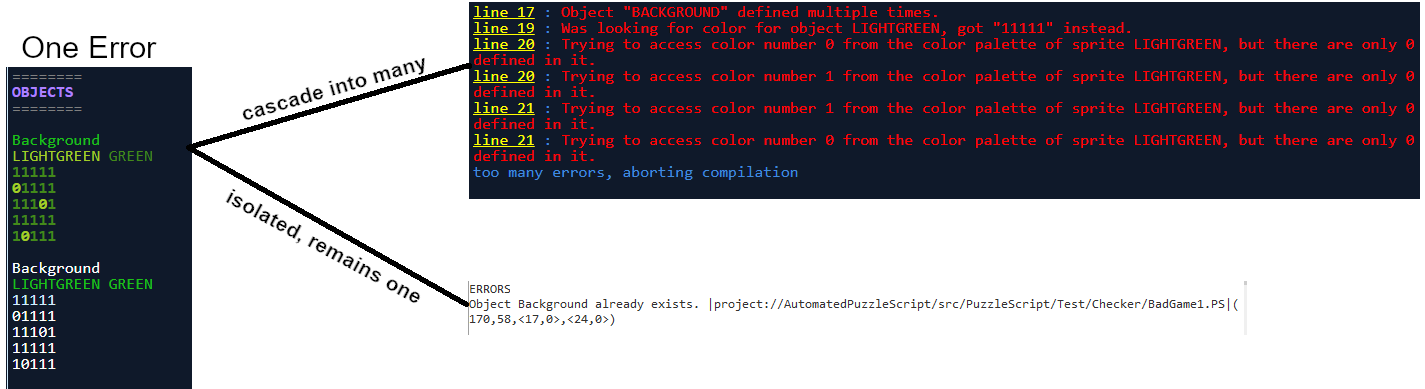
\includegraphics[width=1\textwidth]{images/Example checker.png}
    \caption{Isolation of errors}
    \label{fig:checker_example}
\end{figure}

The JavaScript implementation has 117 unique error/warning messages. This number does not account for messages that appear multiple times. Although our design currently checks for only 72 messages, the discrepancy has two reasons. As previously mentioned, using Rascal's Syntax Definition entails a certain loss of control over the feedback provided in exchange for more readability. The first reason is therefore that a part of these messages are now covered by the general parser failure error intended for the tool designer. The second reason is that, in our design, another part of the messages we extracted from the original implementation have been merged\dd. For instance, the original message has two separate messages to report on an error within the rule depending on whether that error was on the left-hand side or the right-hand side. In our design, these errors are merged into one with a keyword to differentiate the side that raised the error.

\begin{figure}[!t]
    \centering
    \begin{subfigure}{1\textwidth}
        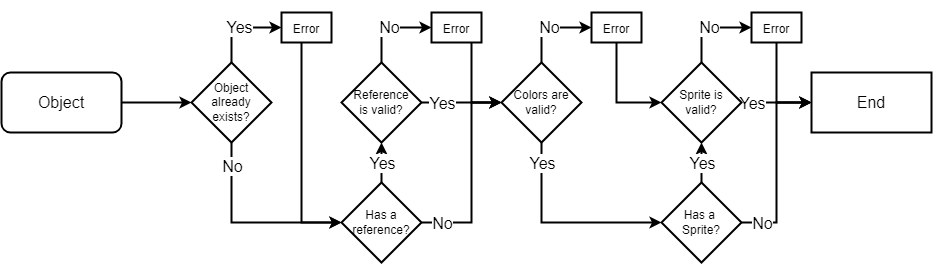
\includegraphics[scale=0.45]{images/checker/Object.png}
        \caption{Flow diagram when validating an Object}
        \label{fig:checker_object}
    \end{subfigure}
    \begin{subfigure}{1\textwidth}
        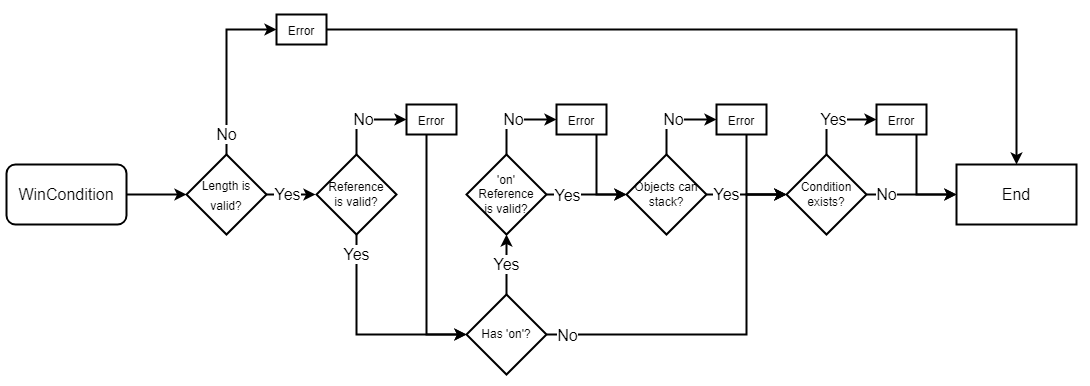
\includegraphics[scale=0.45]{images/checker/WinCondition.png}
        \caption{Flow diagram when validating a WinCondition}
        \label{fig:checker_condition}
    \end{subfigure}
    \caption{Flow diagrams illustrating the validation process done by the checker}
\end{figure}

Figure \ref{fig:checker_object} shows an example of how the checker processes a PuzzleScript component, in this case an Object. Diamonds represent tests that the checker submits the code to and rectangles represent an outcome. This is a simplification of the process that omits specifics on what is considered 'valid'. For instance, a valid color is either a HTML color code or a selection from the color palette selected by the game designer in the prelude. Objects that do not pass the requirement generate an error message that is returned by the checker, to be displayed later. In some cases, an early error causes the remaining checks to be skipped as can be seen in Figure \ref{fig:checker_condition} which illustrates the process for a Win Condition. Figure \ref{fig:checker_remaining} shows how the static checker validates the remaining components of PuzzleScript. Once detected an error is not immediately displayed but rather stored\dd, this serves the dual benefit of making it easy for the IDE to customize how they display the messages and allowing us to centralize our human-readable conversions of these messages. As a result, our redesign is easier to extend in the cases where a tool designers wants to modify the messages. For instance, if a tool designer wants to translate PuzzleScript, all they have to do is go through a single file to have access to the messages. 

In our design, error messages have several different types and subcategories. The main types are \emph{errors} and \emph{warnings}, support for lower categories exist but are currently unused. Generated messages also fall under one of a few sub-categories:
\begin{itemize}
    \item Invalid: The component's syntax is not respected making it unusable
    \item Undefined: The reference/object with that name is never defined but is used
    \item Existing:  The reference/object with that name already exists, but the code is trying to define it again. Sometimes this is generated as an error and sometimes as a warning depending on whether the engine can handle it.
    \item Unused: A warning, the code defines a reference/object/sound but never uses it\dd.
    \item Misc: Very specific errors that do not occur in enough numbers to justify a category
\end{itemize}

We categorize each error with a degree of importance based on whether or not it has a negative impact on the game and its ability to run. Error-level messages can cause issues or unintended side effects in the code that may make the game impossible to resolve, warning-level messages indicate dead or unoptimized code, and information-level messages inform the game designer on gameplay quality and possible best practices. A full list of errors and warnings raised by our tool can be seen in Appendix B. 

\begin{figure}
\vspace*{-4pt}
%\begin{minipage}{0.31\columnwidth}
%\begin{lstlisting}[language=PuzzleScript, xleftmargin=4pt]
%Background
%red green
%11111
%01111
%11101
%11111
%10111
%
%Background
%Red Green
%11111
%01111
%11101
%11111
%10111
%\end{lstlisting}
%\subcaption{duplicate object}
%\end{minipage}
%
%
\begin{minipage}{0.32\columnwidth}
%vRozen: what is Bonk?
\setulcolor{red}
\begin{lstlisting}[language=PuzzleScript, xleftmargin=2pt, , basicstyle=\ttfamily\footnotesize]
Player
black $\color{BurntOrange}orange$ $\color{darkgray}white$ $\color{blue}blue$
$\color{black}.000.$
$\color{black}.$$\color{BurntOrange}111$$\color{black}.$
$\color{darkgray}22222\ul{22222}$
$\color{black}.$$\color{blue}333$$\color{black}.$
$\color{black}.$$\color{blue}3$$\color{black}.$$\color{blue}3$$\color{black}.$
\end{lstlisting}
\setulcolor{black}
% \vspace*{-9.5pt}
\subcaption{Sprite not 5x5}
\setulcolor{black}
\end{minipage}
\hspace{12pt}
%
\begin{minipage}{0.31\columnwidth}
\setulcolor{red}
\begin{lstlisting}[language=PuzzleScript, xleftmargin=4pt,  basicstyle=\ttfamily\footnotesize]
####
#.O#$\ul{..}$
#..#$\ul{\#\#..}$
#@P.$\ul{.\#}$
#..*
#..#$\ul{\#\#}$
####$\ul{..}$
\end{lstlisting}
\subcaption{Uneven level rows}
\setulcolor{black}
\end{minipage}
\hspace{12pt}
\begin{minipage}{0.28\columnwidth}
% \setulcolor{Gold}
\begin{lstlisting}[language=PuzzleScript, xleftmargin=4pt, basicstyle=\ttfamily\footnotesize]
Crate
$\color{BurntOrange}orange$ $\color{Green}\ul{green}$
$\color{BurntOrange}00000$
$\color{BurntOrange}0$$\color{black}...$$\color{BurntOrange}0$
$\color{BurntOrange}0$$\color{black}...$$\color{BurntOrange}0$
$\color{BurntOrange}0$$\color{black}...$$\color{BurntOrange}0$
$\color{BurntOrange}00000$
\end{lstlisting}
\subcaption{Unused color}
\setulcolor{black}
\end{minipage}
\medskip

\begin{minipage}{\columnwidth}
%, xleftmargin=4pt, basicstyle=\ttfamily\scriptsize]
\setulcolor{red}
\begin{lstlisting}[language=PuzzleScript, basicstyle=\ttfamily\footnotesize]
[Eyeball| ... |Player] -> $\ul{[> Eyeball|Player]}$
\end{lstlisting}
\vspace*{-4pt}
\subcaption{Missing ellipsis in right hand side of rule}
\setulcolor{black}
\end{minipage}
\medskip

\begin{minipage}{\columnwidth}
%, xleftmargin=4pt, basicstyle=\ttfamily\scriptsize]
\setulcolor{red}
\begin{lstlisting}[language=PuzzleScript, xleftmargin=10pt, basicstyle=\ttfamily\footnotesize]
[> Player|Crate] -> [> Player] $\ul{[> Crate]}$
\end{lstlisting}
\vspace*{-4pt}
\subcaption{Unexpected rule part in right hand side of rule}
\setulcolor{black}
\end{minipage}

\caption{Errors and warnings detected by the checker}
\label{fig:ErrorsWarnings}
\vspace*{-8pt}
\end{figure}

As we previously mentioned, our tool raises errors and warnings that do not exist in the original implementation. Part of these messages are merges and others are brand news\dd. A sample of these new messages is displayed in Table \ref{tab:new_errors}. Many of these messages reference existing objects that are never used. Unused objects present two issues. The first issue is that unused objects represent dead code that inflate the file size but add no value. Dead code adds unnecessary complexity to the codebase and makes it more difficult to understand. The second issue is that unused objects may also give a false impression of the game. This false impression of the game makes it hard for other game designers to understand the design of the game. Our tool also raises a warning when redundant components are implemented into the game. For instance, duplicate win conditions can happen when game designers are not fully aware of what object a legend references. This can cause them to create duplicate instances through the use of different legends referencing the same item. Finally, ScriptButler performs additional checks on Win Conditions, an area left relatively untouched by the original implementation. We design checks to ensure that game designers do not accidentally write conditions that are mutually exclusive.

\begin{table}
\centering
\caption{New errors in ScriptButler}
\label{tab:new_errors}
\begin{tabular}{l|l|l}
Name                               & Type    & Message                                                                                                                    \\ \hline
existing\_sound                    & Warning & \begin{tabular}[c]{@{}l@{}}A sound event has already been \\ registered for this object with \\ these actions\end{tabular} \\
existing\_condition                & Warning & \begin{tabular}[c]{@{}l@{}}A victory condition similar to \\ this one already exists\end{tabular}                          \\
existing\_rule                     & Warning & \begin{tabular}[c]{@{}l@{}}A rule similar to this one already \\ exists\end{tabular}                                       \\
impossible\_condition\_unstackable & Error   & \begin{tabular}[c]{@{}l@{}}A victory condition requires items \\ existing on the same layer to stack\end{tabular}          \\
redundant\_prelude\_value          & Warning & \begin{tabular}[c]{@{}l@{}}This prelude keyword does not \\ require a value\end{tabular}                                   \\
unused\_colors                     & Warning & \begin{tabular}[c]{@{}l@{}}This object defines more colors \\ than it uses\end{tabular}                                    \\
unused\_object                     & Warning & This object is defined but never used                                                                                      \\
unused\_legend                     & Warning & This legend is defined but never used                                                                                     
\end{tabular}
\end{table}

The result of this phase is a list of messages reporting on the state of the game's code. The intent is for those messages to be passed on to the IDE and displayed to the user as shown in \ref{fig:ErrorsWarnings}. The game designer gains a complete overview of the game code and an understanding of its current flaws. Once the designer has resolved the errors, the game code is passed to he compiler. The compiler is discussed in the next section.


\subsection{Compiler}
Game languages require compilers to optimize their performance. Compilers transform the code into lower-level machine code. For PuzzleScript, this means converting the DSL into Rascal data structure. ScriptButler already does part of this task during the parsing, the compilation process completes it. The compiler transforms the existing data structures further, this increases performance but reduces readability. The new data structures do not resemble the original code at all. It may even be impossible to generate code back from the compiler because the structure is lost. For instance, the compiler resolves all references, replacing them with the list of object referenced. As a result, the original reference is lost. Our compiler is separated into three phases, representing the three sections that need to be compiled. Sounds are not compiled because they are not implemented. Objects are not compiled because our tool only requires their name. As such, we only compile three sections: Win Conditions, Levels, and Rules. All three are explained in detail below.

\subsubsection{Levels}
In PuzzleScript, game designers create 2D representations of their levels with the use of legend and aggregates. However, levels are actually 3-dimension when factoring in the collision layer. As a result, we compile the levels into 3D arrays. The design decision we have to take is in which order to arrange the array and their relation to the coordinates. Each object on a level has an XYZ coordinate. X represents the row, Y the column, and Z the layer they are present on. Each of these triples is unique. We have two choices, we can either store the levels as a XYZ array or as a ZXY array. A XYZ array is an array where the first dimension represents the X coordinate, the second the Y coordinate and the third the Z coordinate. An XYZ array has a similar concept but in a different order. The order matters depending on how we match the rules. We decided on an ZXY\dd design, where the first dimension is the layer. This makes it easier to build the level layer by layer. Using the other method would allow us to build levels one row at a time but makes it harder to check using our rule system.

Levels are designed to be able to function standalone. Each level stores all the data required to function. Only the rules and win conditions are required to run a level. However, to render a level, the engine also provides access to the object sprite even if it does not use it currently. During compilation, references and aggregation are resolved and a background layer is generated for rendering purposes. The data structure makes it possible for the engine to store the contents of a level in a simple structure.

\subsubsection{Win Conditions}
Compiling win conditions is a simple process. We resolve references and store them in data structure that makes it easier to check against the 3D structures representing our levels. Levels are also compiled in a way that allows the engine to check for their contents efficiently. Because we store the contents of a level in a simple structure, we can easily check the prerequisites of certain win conditions. For instance, if a level does not contain any instance of ObjectX then the condition \texttt{'No ObjectX on ObjectY'}. This helps performance as it does not require us to go through the level pixel by pixel. The engine can simply access the list of objects contained in the level and make assumptions based on that. However, if there is an instance of ObjectX present, we then have to conduct the more expensive check.

\subsubsection{Rules}
Rules are the most complex part of PuzzleScript and we aim to simplify them in ScriptButler. This goal means that we aim to make the system simpler to extend and we make the rules simpler to debug from a game designer perspective. To this end, we leverage a feature of PuzzleScript called Abstract Patterns\footnote{\url{https://tutor.rascal-mpl.org/Rascal/Patterns/Abstract/Abstract.html}}\dd. Abstract Patterns can be used to match the code with patterns. We use it to match data structure representing a level. However, Rascal does not have native support for creating these Abstract Patterns. The patterns are intended to be used statically to match specific code patterns. We need to be able to generate Abstract Patterns from the Rules written by game designers. We achieve this by generating Abstract Patterns as code to be interpreted by our engine\dd. This design decision incurs a performance loss, as the Rascal code is not compiled but interpreted.

Figure \ref{fig:Rule Compilation Code} shows a simple Rule written in PuzzleScript. This rule allows the player to push a crate. Using our compiler, we transform the rule into a Rascal Abstract pattern that can be seen in \ref{fig:Rule Compilation Pattern}. The pattern represents a 3D array similarly to the compiled form of a Level. In this instance, the game has three layers, as such the first dimension of the array is three elements long. However, the objects referenced in the original layer only exist on the third layer. As such, the first two layers (lines 2 and 3) match for anything and then pass the match to the replacement, changing nothing. Line 4 and 5 unpack the second and third dimension of the level, ensuring that whatever comes after and before the match is passed to the replacements pattern. Finally, lines 6 and 7 handle the actual matching. Line 7 matches a player moving in a direction and Line 8 matches a crate standing still. A similar pattern is used to replace the crate with a moving crate.

\begin{figure}[!t]
    \begin{subfigure}{1\textwidth}
        \begin{lstlisting}[language=rascal]    
        1 # [ 
        2 #     [ *layer0 ], 
        3 #     [ *layer1 ], 
        4 #     [ *prefix_lines2, 
        5 #         [ *prefix_objects2, 
        6 #             Object player0 : moving_object(str name0_0_2 : /player/, int id0_0_2, str direction0_0_2 : relative_right, Coords coords0_0_2 : <xcoord0, ycoord0, zcoord0_0_2>), 
        7 #             Object crate0 : object(str name1_0_2 : /crate/, int id1_0_2, Coords coords1_0_2 : <xcoord1, ycoord1, zcoord1_0_2>), 
        8 #         *suffix_objects2 ], 
        9 #     *suffix_lines2 ]
        10# ]
        \end{lstlisting}
        \vspace*{-8pt}
        \caption{An abstract pattern of the rule in Figure \ref{fig:Rule Compilation Code}}
        \label{fig:Rule Compilation Pattern}
    \end{subfigure}
    
    \begin{subfigure}{1\textwidth}
        \begin{lstlisting}[language=PuzzleScript]
        [ >  Player | Crate ] -> [  >  Player | > Crate  ]
        \end{lstlisting}
        \vspace*{-8pt}
        \caption{A simple PuzzleScript Rule allowing pushing Crates}
        \label{fig:Rule Compilation Code}
        \vspace*{-8pt}
    \end{subfigure}
    
    \caption{Compiling rules}
    \label{fig:compiling rules}
\end{figure}

The compiler requires multiple passes to compile a rule into a list of abstract patterns. However, the end result is more readable from the perspective of a tool designer. Our aim with this design decision is to make it easier to extend PuzzleScript with additional features in rules. Validating Abstract Patterns is easier than validating functions like the original implementation generates. 

The result of the compiler is a list of data structures for Win Conditions, Rules and Levels which can be run by the engine. The data structures we compile are easier to extend than the original implementation. This decision does not change anything for the game designer besides a performance impact caused by the new design focus on extensibility and maintainability. 

\subsection{Engine}
We divide the game loop into additional phases to avoid unnecessary coupling. We make it so that the phases only require the necessary data to be passed\dd, as opposed to passing the entire game. Figure \ref{fig:engine_flow} shows a full flow diagram of the engine, we briefly explain the different phases below:
\begin{itemize}
    \item Plan Move: Mark player objects as needing to be moved if the player has given a move command
    \item Apply Rules: Apply the rules as many times as possible
    \item Do Move: Move all objects marked as such, if there is an obstacle, see if we can move that obstacle
    \item Apply Late Rule: Apply the late rules as many times as possible.
    \item Check Victory: Check if we meet all the victory conditions, if not, do the loop again
\end{itemize}

The engine provides support to the game loop in the form of individual functions\dd. The game loop we design uses those function to run the game. We made this design decision to make it simple for other developers to create their own version of the loop by assembling the functions in a different order. Tool developers can also override the function to inject their changes without modifying the loop. For avoiding infinite loops, users can specify a limit on the number of times a rule can be applied.

\begin{figure}[!t]
    \centering
    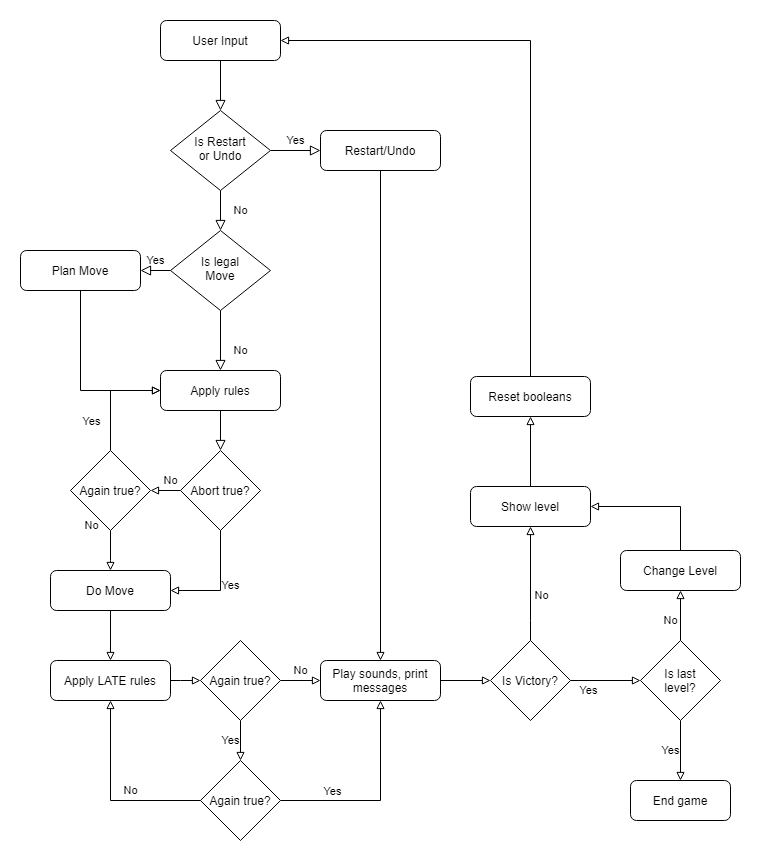
\includegraphics[width=1\textwidth]{images/Engine Flow.drawio.png}
    \caption{Engine flow graph}
    \label{fig:engine_flow}
\end{figure}



\section{Extending our implementation}
We extend the design of our PuzzleScript implementation with several features to support iterative game design. First, we design a dynamic analyzer that provides the game designers with feedback on their gameplay. Second, we implement a plugin that provides syntax highlighting and error reporting within Eclipse. Finally, we design a user-facing interface using Salix to run games. Below, we detail these functionalities one by one. 

\subsection{Dynamic Analyzer}
Our dynamic analyzer phase runs after the engine phase, allowing game designers to gather gameplay-related feedback. The phase runs subsets of the compiled code in the background when the project is built. This process is more expensive than a static check but not required as often. Messages are generated the same way as the static checker and can be manipulated similarly by IDEs.

We perform two types of dynamic analysis, standard dynamic analysis that checks for general gameplay quality and "trivial solutions". The standard dynamic analysis either checks components individually or by seeing how a few different ones interact together. Our "trivial solutions" follow in the line of thinking of our original questions on the complexity of finding fun. Finding a solution to a level is similarly complex, checking if a level can be solved is more of an AI question. Our design makes it possible to implement an AI plugin to solve this problem but that is not the focus of this thesis. Therefore, instead of trying to determine if a game is fun by checking if a level is solvable in an interesting way, we make check whether a game could be unfun by checking if a level is solvable using uninteresting solutions.

Currently, two trivial solutions exist:
\begin{itemize}
    \item Unidirectional: Is it possible to win the level by only going in one direction
    \item Unruled: Is it possible to win the level without using any rules.
\end{itemize}

\textbf{Unidirectional} is done by running a level in the background with the four directional inputs. If after submitting the length of level times two in inputs the level is not won then it is not considered \textbf{unidirectional} in that direction. If none of the four inputs come up positive, the level passes. For \textbf{unruled}, we use the compiled version of Levels and WinConditions to check whether all objects required are present on the map. This does not, however, check if they are reachable, simply whether they are present or not. 

When performing our standard dynamic check, we verify the following:
\begin{itemize}
    \item Instant Victory: Is the win condition already fulfilled for the level before player interaction
    \item Impossible Victory: Does the win condition require objects that are not present and not supplied by any rules
    \item Rule Similarity: A deeper check where we compare the compiled forms of the rules to see if they are similar
    \item Metrics: We provide various metrics to the game designer that might be useful. This data is provided without analysis to avoid possible misinterpretation. 
    \item Unusable Rule: Similarly to Impossible Victory, we check whether the prerequisites for a rule can be spawned by another rule. 
\end{itemize}

Our dynamic analysis is done similarly to our static checking, it is its own phase, but instead of taking an AST of the game, it takes a compiled engine. The same maintainability and extensibility principles apply as with the rest of the tool. Adding more dynamic checks is a simple matter of writing the logic, adding messages and calling the logic from the main function. The result is also similar, a list of messages to be manipulated as the tool designer desires. The common next step is to display those messages in the IDE.

\subsection{IDE}
\label{sec:ide}
% Explain how we integrated our language to IDE, don't make it too much of a big deal though since it only works with Eclipse. 
ScriptButler offers an IDE plugin integrated within Eclipse. This plugin leverages the fact that Rascal's Eclipse integration. Using simple code we add an outline, syntax coloring, a contextual menu, and log messages. We aim to support game designers by providing more features than the IDE from the original implementation. As a reminder, the original implementation provides syntax coloring and partial error reports. Additionally, it also provides features that allow game designers to share and export their games. However, we specifically focus on tools that provide support for game designers in their explanation of the design space.

The first feature that ScriptButler's IDE provides is syntax coloring. This feature already exists within the original implementation. In our design, we tie it to the parse tree annotations\dd. Users can change the coloring without having to change the code of the grammar or mess around with regular patterns. Additionally, this decision is important because the annotations are generated dynamically during the post-processing phase. Syntax coloring improves readability and provides context to the code\cite{DBLP:conf/ppig/Sarkar15a}. Additionally, in the case of PuzzleScript we color the sprites to provide game designers with a preview of the sprite's appearance.

% \begin{figure}[!t]
%     \centering
%     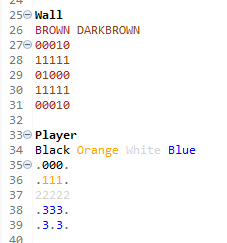
\includegraphics[width=0.50\textwidth]{images/Syntax_colouring.png}
%     \caption{Syntax highlighting}
%     \label{fig:ide_colouring}
% \end{figure}

The second feature is an outline view\dd. An outline view is a separate window the game designer can open to gain an overview of their game's contents. This feature allows the game designer to quickly navigate the file based on its contents. For instance, if a designer desires to return to the code for a specific object, they can simply click on that object's name in the outline. The outline improves the efficiency of the designer, especially as the file size grows. The outline we design provides an overview and a navigation shortcut for all major components of PuzzleScript. Tool designers can easily extend this outline to provide an overview of smaller components or to display additional data. Figure\ref{fig:ide_outline} shows this outline view with all branches expanded.

\begin{figure}[!t]
    \centering
    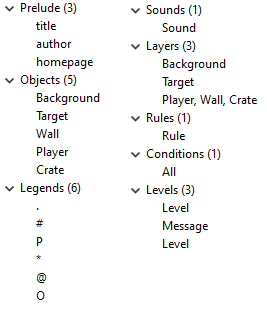
\includegraphics[width=0.5\textwidth]{images/Example_outline.png}
    \caption{IDE Outline}
    \label{fig:ide_outline}
\end{figure}

The third feature of the IDE is the display of error messages. In the original implementation, messages just appear in the console after compilation. However, this kind of implementation does not scale well with high number of messages. As such, we design ScriptButler's IDE so that it display the error messages right next to the code line creating the issue. Figure \ref{fig:ide_messages} shows this design implemented. The final feature of the IDE is a contextual menu. This contextual menu provides game designers with the ability to start up the Web GUI straight from the editor. However, the feature is very extensible and can be used for a wide variety of actions. For instance, it should be possible to use it to export the game or share it online. 

\begin{figure}[!t]
    \centering
    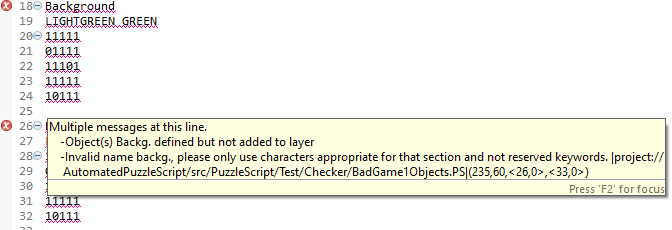
\includegraphics[width=0.85\textwidth]{images/Rascal_IDE.png}
    \caption{IDE Messages}
    \label{fig:ide_messages}
\end{figure}


In conclusion, ScriptButler's IDE provides game designers with an editor to interact with the tool itself. This editor supports game designers with a wide variety of features that make programming more efficient.




\subsection{Running Games}
ScriptButler offers game designers the ability to run their game in a browser. In the original implementation, this feature is coupled with the editor. However, we separate it and extend its capabilities to provide playtesting support using a \emph{salix} web app. At its heart, the salix web app provides game designers the ability to run their game and to see it graphically represented through a Web GUI. We use the Web GUI because Rascal does not possess the feature to represent the game graphically or to 'wait' for user input. We leverage this weakness as a strength by also extending the Web GUI with useful playtesting tools. 

The GUI provides a list of victory conditions and whether or not they are true in the current level state. Game designers can use this feature to check their assumptions of what their victory conditions are. They can create a level state where they think certain conditions should be true and then check whether or not they actually are. The GUI also provides a list of rules, how many times they were used in the last turn and what they look like when compiled. The last part is probably more useful to engine developers, which is why it's hidden from sight by default. Game designers can use this feature to check whether the rules actually run when they intend them to, and how many times they match. Finally, the GUI provides game designers with a \emph{'layered'} view of their level. A 'layered' view is a representation of the level where objects are separated based on which collision layer they appear on. This feature provides an easy way for users to see all objects on a particular pixel that may otherwise be hidden by objects they are stacked under.

The Web GUI provides tool to support the game designers when they debug their games. It uses salix which means it is, for a majority, written in Rascal. This design decision makes it easier to edit for those seeking to modify or extend the tool. The downside to our approach is that salix is still a relatively new library and suffers in regard to response times. Figure \ref{fig:salix_webserver} shows an example of Web GUI's appearance. 

\begin{figure}[!t]
    \centering
    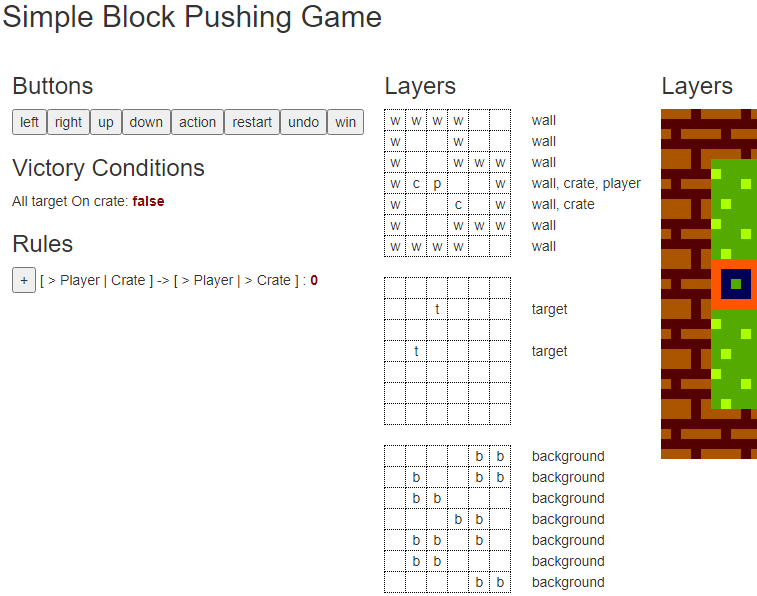
\includegraphics[width=1\textwidth]{images/Rascal Salix.png}
    \caption{Salix web app}
    \label{fig:salix_webserver}
\end{figure}
\section{Testing}
\label{sec:testing}
%  Explain unit tests conducted in this project
Here we describe an extensive test suite that verifies ScriptButtler's implementation works according to its design. We describe how the suite tests different parts of the tool and what the test results are. We validate and verify our tool using two separate methods. We describe validation Chapter \ref{ch:case} and verification in this chapter. The test suite consists of a dozen sections that test each section of our PuzzleScript implementation. The tests can be found on the GitHub repository\footnote{\url{https://github.com/ClementJ18/Rascal-PuzzleScript/tree/main/src/PuzzleScript/Test}}.

Each section consists of several PuzzleScript files containing mock data and one Rascal file that conducts the tests. The test files are intended to either verify correctness or error handling. Verifying correctness consists of running valid code through the section we are testing. Verifying error consists of running invalid code and testing to see if a controlled error message is raised. The test files consist of mock data which represent games, sections and atomic components of PuzzleScript. The complexity of the mock data varies based on the test requirements.

\paragraph{Parser}
The test suite verifying the Parsing phase is the most extensive but also has the simplest mocking data. We test individual elements of a game such as objects, rules parts and levels; complete sections and full games. We test for the correctness of this phase by checking whether or not our grammar successfully parses the mock data. Conducting additional tests to verify the integrity of the parsed data during this phase is unnecessary, the data is verified in future phases. In the cases where the parsed data is invalid, then the Abstract Syntax Tree (AST) itself will raise an error, therefore, we verify the parsed data in the phase where we verify the AST. We reuse the mock data from the parsing test suite quite frequently as mock data for our other test suites. 


\paragraph{Static Checker}
The next suite performs verification on the functionality of the static checker by purposefully triggering errors. The mock data consists of sections of PuzzleScript games plus a few additional cases that do not fit in any particular section. Throughout our test suite, we also have mock data which specifically focus on getting a correct result, and this mock data is used both for verification and to guide us during development.

\paragraph{Test-Driven Development}
Our approach to development is test-driven, so we develop by designing tests first and then writing code that passes those tests. Test-driven development requires the test suite to be designed with intent. We focus on creating tests that provide coverage for both high-level and low-level functions.  The test suite grows in complexity as it progresses through the phases of compilation. The time running the suite takes also increases as the tests run increasingly more code. Running tests for the dynamic analysis phase is the most expensive currently.

\paragraph{Results}
Running our tests gives us feedback on the quality of our tool's source code. ScriptButler is able to parse and statically check the majority of valid source code with an insignificant amount of incorrect error reporting. However, the tool struggles when it has to parse code that has severe structural issues. This causes exception in the runtime of the tool usually resulting in a crash. There is no application with native support for counting of code lines in Rascal. However, we can use \emph{cloc} and count it as if it was Java code to get an estimate. The core of our PuzzleScript implementation totals 9 files and 2317 lines of code. As a reminder, PuzzleScript's official implementation had 3 core files that totaled 5820 lines of code. In Table \ref{tab:test_suite_results} we show the number of tests associated with each section and the percentage of those tests that pass. Note that some tests are used in multiple phases. If a phase does not have any test files, then that means it reuses mock data from previous phases.

\begin{table}
\centering
\caption{Results of our test suite}
\label{tab:test_suite_results}
\begin{tabular}{l|l|l|l|l}
Phase            & \# of test files & \# of tests & Tests passed & Comments                                                                                               \\ \hline
Parser           & 28               & 28          & 24/28        & \begin{tabular}[c]{@{}l@{}}Failing tests all relate to \\ comment parsing\end{tabular}                 \\
Post-processing  & 0                & 16          & 15/16        & \begin{tabular}[c]{@{}l@{}}Failing test relates to comment \\ parsing\end{tabular}                    \\
Checker          & 9                & 9           & 9/9          &                                                                                                        \\
Compiler         & 0                & 0           & 0/0          & \begin{tabular}[c]{@{}l@{}}Verified through the engine \\ behavior\end{tabular}                       \\
Engine           & 11               & 12          & 10/12        & \begin{tabular}[c]{@{}l@{}}Advanced games do not properly \\ run\end{tabular}                          \\
Dynamic Analyser & 7                & 6           &              &                                                                                                        \\
IDE              & 1                & 1           & 1/1          &                                                                                                        \\
Interface        & 0                & 1           & 1/1          &                                                                                                        \\
Comment Parsing  & 7                & 7           & 6/7          & \begin{tabular}[c]{@{}l@{}}Tests are relatively simple, not\\ representative of all cases\end{tabular} \\
General Parsing  & 83               & 1           & 72/83        & \begin{tabular}[c]{@{}l@{}}Only tests whether games parse, \\ no data validation\end{tabular}              
\end{tabular}
\end{table}


\begin{figure}[ht]
    \label{fig:checker_remaining}
    \begin{subfigure}{1\textwidth}
        \centering
        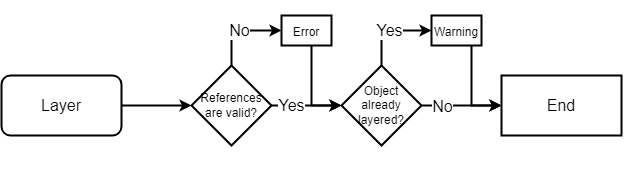
\includegraphics[scale=0.45]{images/checker/Layer.png}
        \caption{Flow diagram when validating a Layer}
    \end{subfigure}
    \begin{subfigure}{1\textwidth}
        \centering
        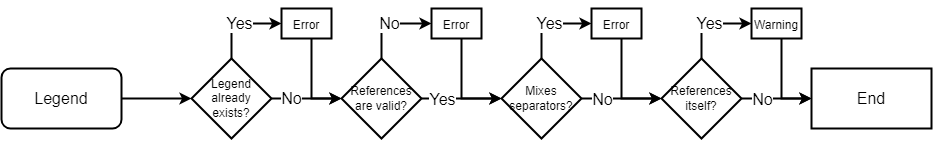
\includegraphics[scale=0.45]{images/checker/Legend.png}
        \caption{Flow diagram when validating a Legend}
    \end{subfigure}
    \begin{subfigure}{1\textwidth}
        \centering
        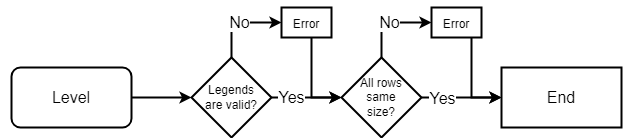
\includegraphics[scale=0.45]{images/checker/Level.png}
        \caption{Flow diagram when validating a Level}
    \end{subfigure}
    \begin{subfigure}{1\textwidth}
        \centering
        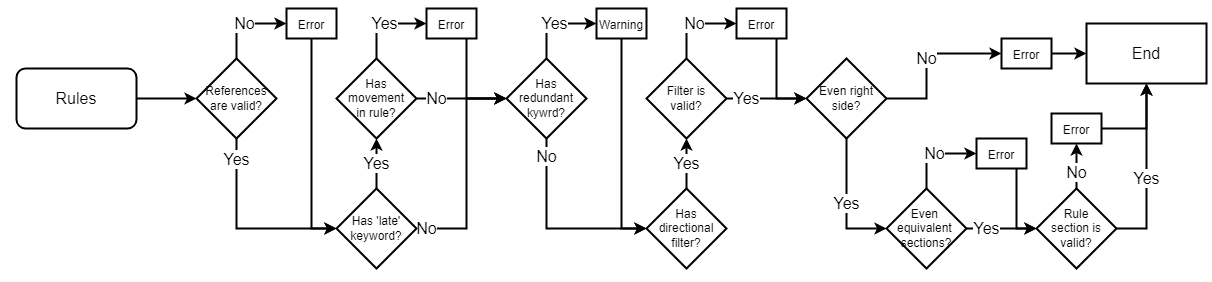
\includegraphics[scale=0.55]{images/checker/Rule.png}
        \caption{Flow diagram when validating a Rule}
    \end{subfigure}
    \begin{subfigure}{1\textwidth}
        \centering
        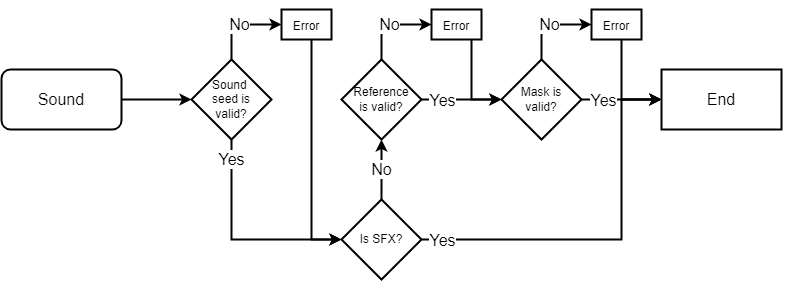
\includegraphics[scale=0.45]{images/checker/Sound.png}
        \caption{Flow diagram when validating a Sound}
    \end{subfigure}
    \caption{Flow diagrams for checker validation.}
\end{figure}